\documentclass[11pt, a4paper]{article}

% --- 宏包加载 ---
\usepackage[utf8]{inputenc}
\usepackage{ctex} % 支持中文
\usepackage{geometry}
\geometry{left=2.5cm, right=2.5cm, top=2.5cm, bottom=2.5cm}
\usepackage{amsmath, amsfonts, amssymb} % 数学公式
\usepackage{graphicx} % 插入图片
\usepackage{booktabs} % 表格
\usepackage{listings} % 插入代码
\usepackage{xcolor}
\usepackage{float} % 控制图片位置 [H]
\usepackage{hyperref} % 超链接

% --- 代码样式设置 ---
\lstset{
    basicstyle=\ttfamily\small,
    keywordstyle=\color{blue},
    commentstyle=\color{gray},
    stringstyle=\color{orange},
    breaklines=true,
    frame=single,
    language=Python
}

% --- 标题信息 ---
\title{基于 NetVLAD 与特征匹配的图像检索实验报告}
\author{张宗桪\\ 学号:2023K8009991013}
\date{\today}

\begin{document}

\maketitle

\section{实验目的}
\begin{enumerate}
    \item 掌握深度学习图像检索流程,理解 NetVLAD 聚合层的工作原理。
    \item 比较基于深度学习的描述子 (SuperPoint) 在不同场景下的匹配鲁棒性。
    \item 分析光照变化、大角度旋转对特征匹配性能的影响。
\end{enumerate}

\section{实验原理}

\subsection{NetVLAD 图像检索}
NetVLAD 是将局部特征聚合为全局描述符的经典方法。其核心在于计算局部特征 $\mathbf{x}_i$ 与聚类中心 $\mathbf{c}_k$ 的残差累加:
\begin{equation}
V(j, k) = \sum_{i=1}^N \frac{e^{\mathbf{w}_k^T \mathbf{x}_i + b_k}}{\sum_{k'} e^{\mathbf{w}_{k'}^T \mathbf{x}_i + b_{k'}}} (\mathbf{x}_i[j] - \mathbf{c}_k[j])
\end{equation}
本实验中,我们使用 VGG16 作为后端的特征提取网络,提取 $512$ 维特征图。

\subsection{特征匹配方法}
本实验采用了superpoint方法:
\\SuperPoint 由 Magic Leap 团队于 2018 年提出。它是一个全卷积神经网络(CNN),专门设计用于实时提取特征点和描述子。 SuperPoint 网络结构包括两个主要部分:关键点检测器和描述子生成器。关键点检测器通过一个卷积层输出一个热图,表示图像中每个像素点作为关键点的概率。描述子生成器则通过多个卷积层提取每个关键点的局部特征,并将其映射到一个高维空间中,生成描述子。

\section{实验设置}

\subsection{数据集说明}
自采数据集包含以下两组场景:
\\1. 室内场景:采集自寝室 包含低光照和大角度旋转情况的图像。
\\2. 室外场景:采集自教学楼 包含相似情况的图像。
\begin{figure}[H]
    \centering
    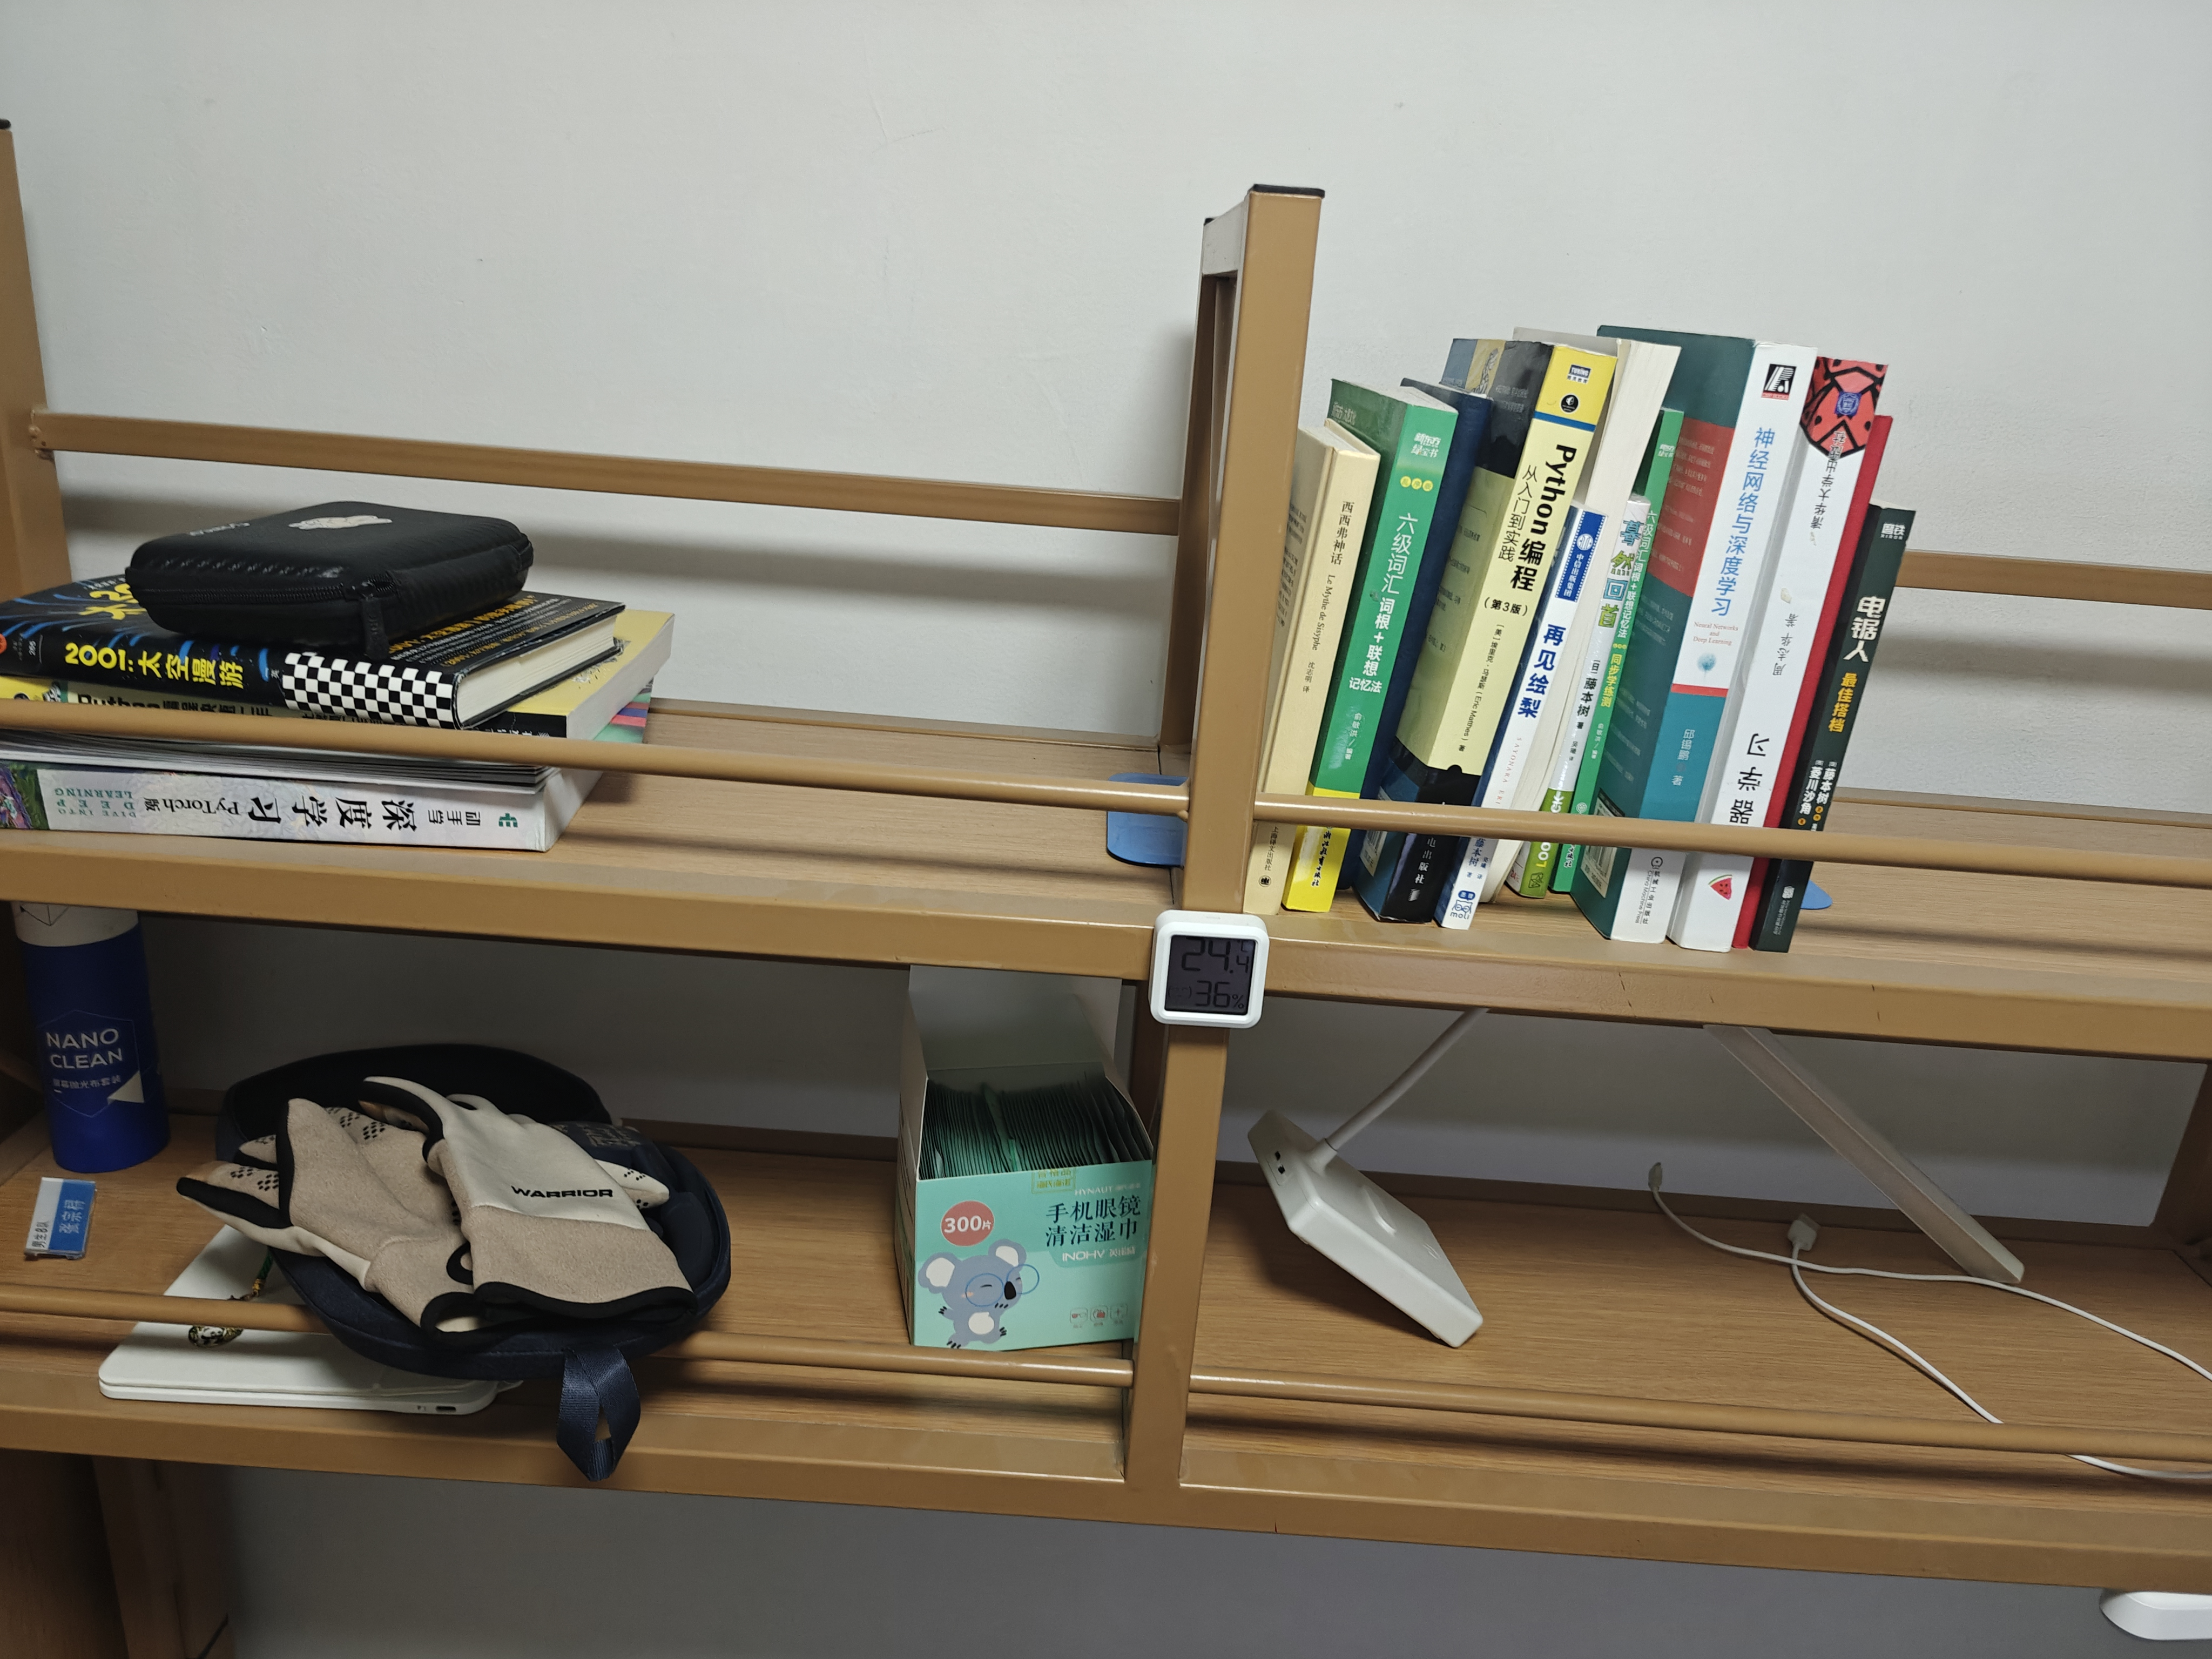
\includegraphics[width=0.8\textwidth]{./data/retri2/sources/5.jpg}
    \caption{室内场景示例图}
\end{figure}
\begin{figure}[H]
    \centering
    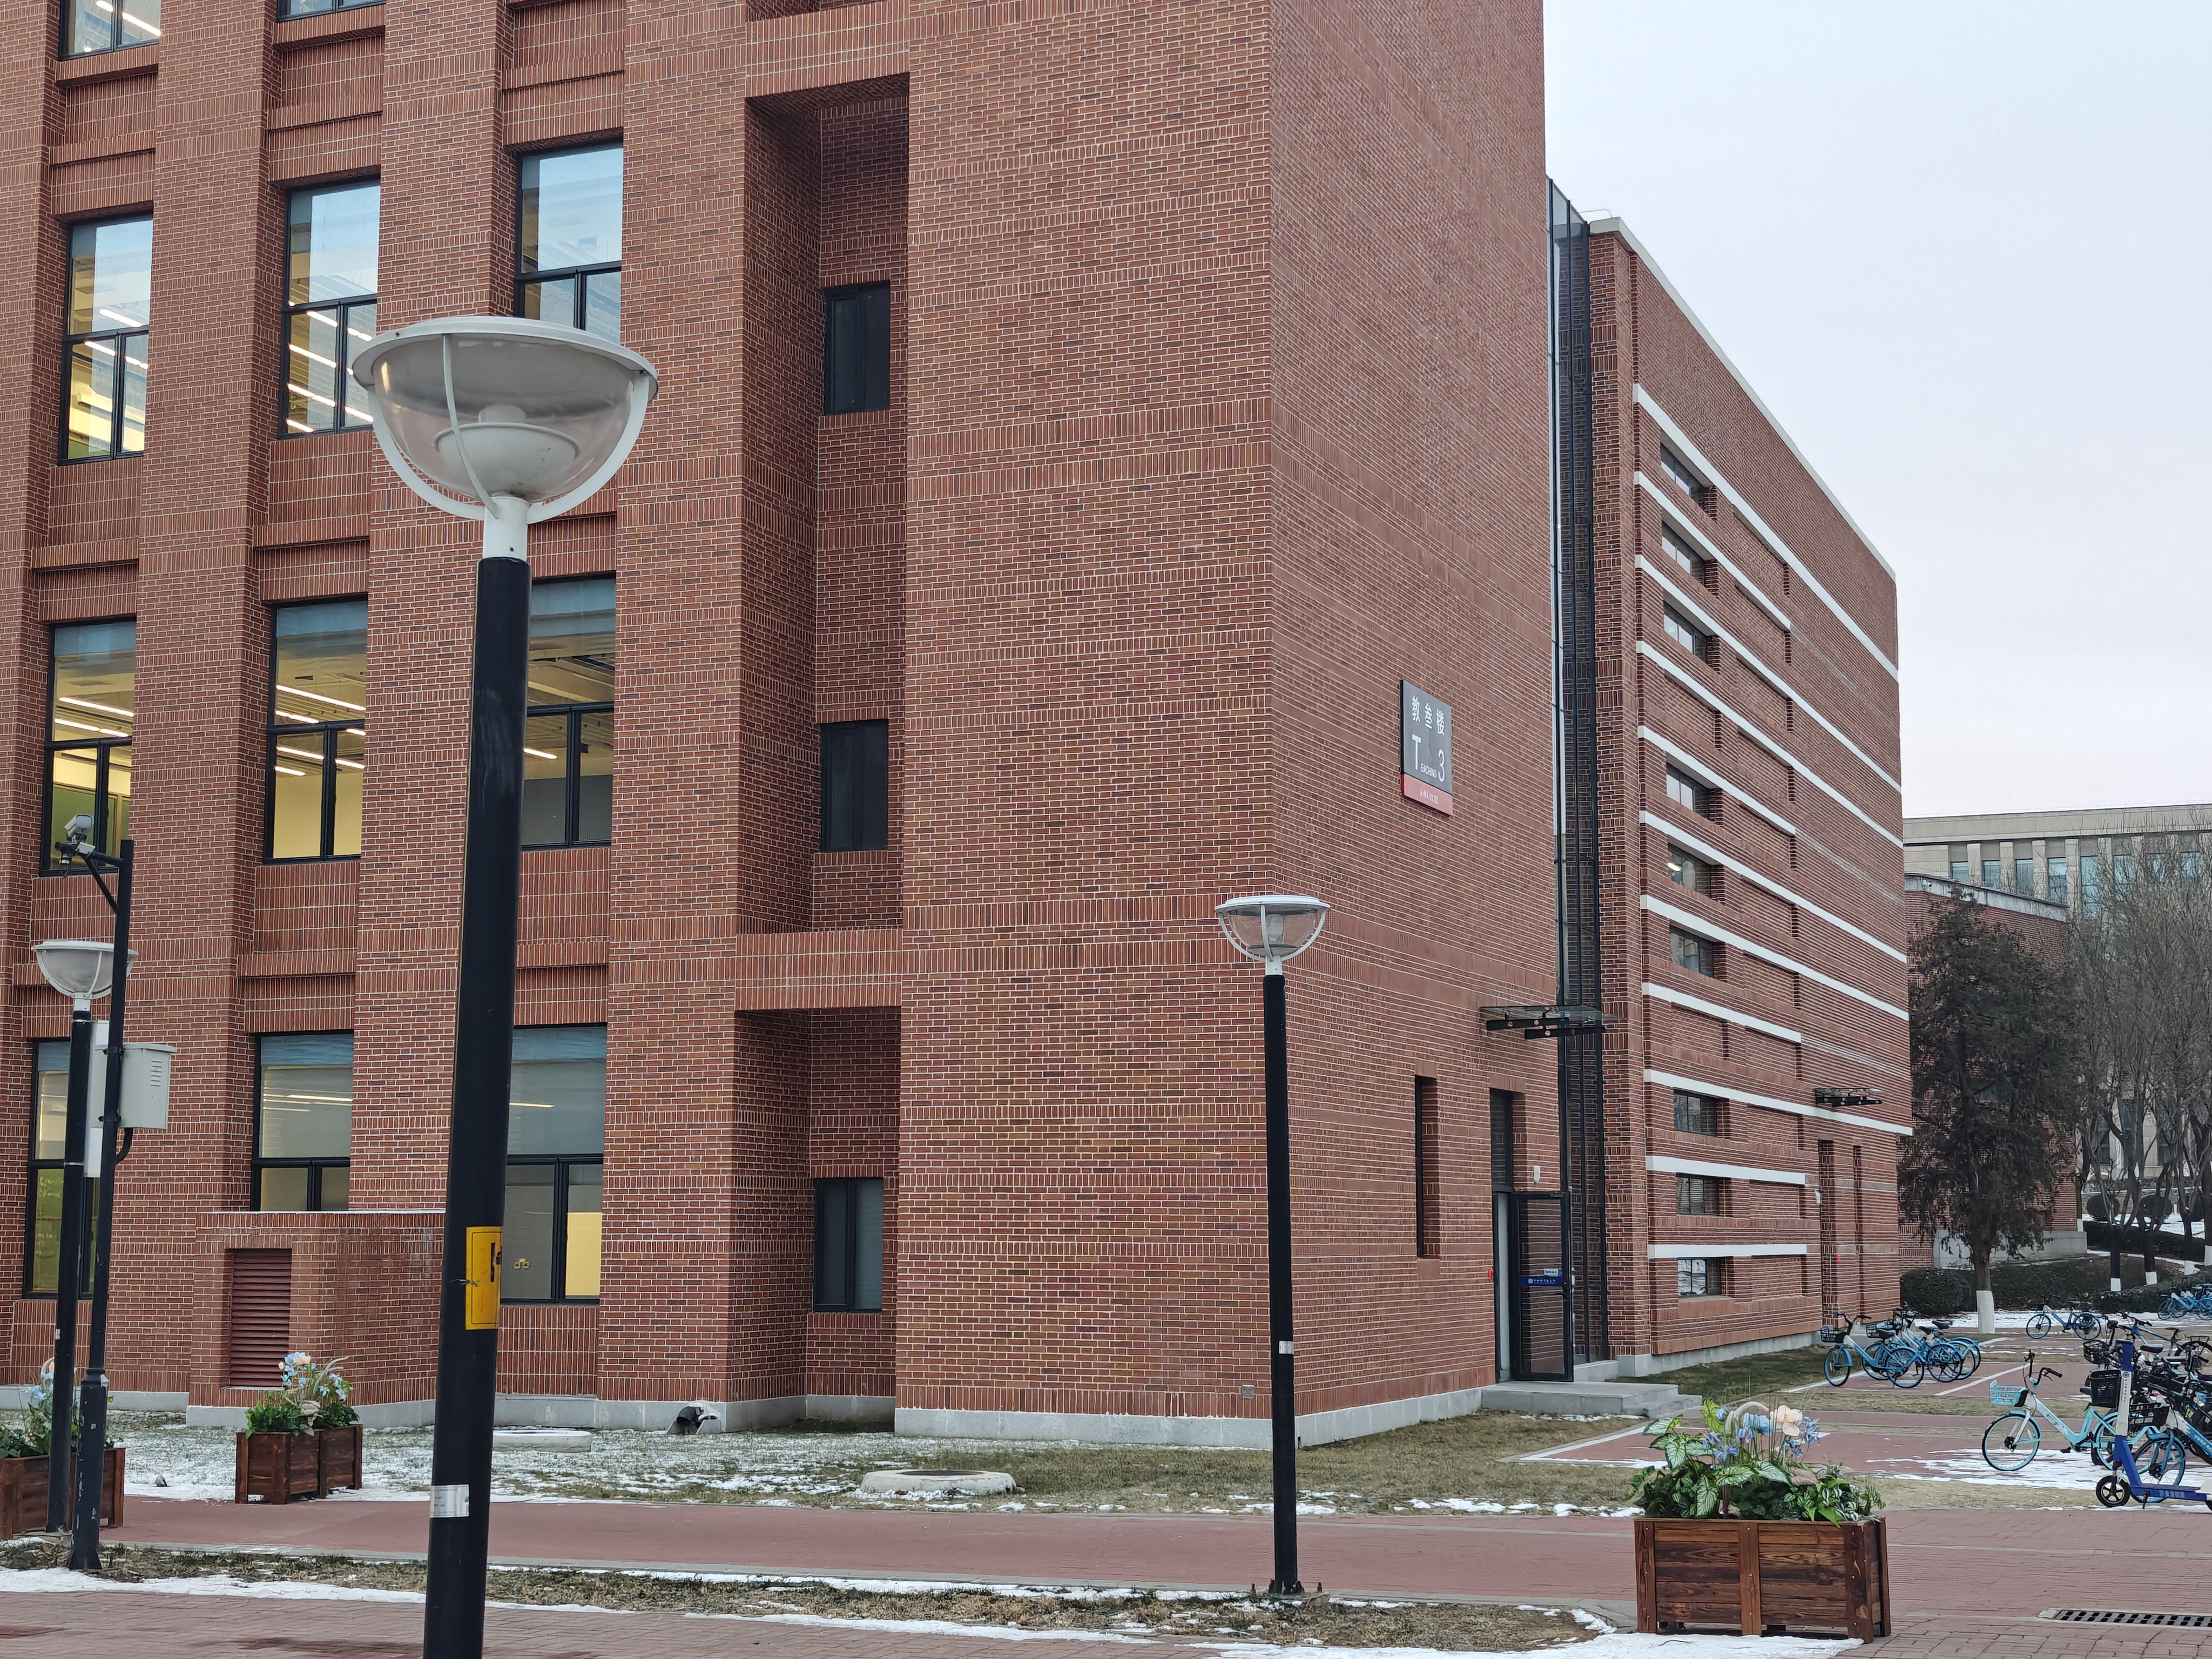
\includegraphics[width=0.8\textwidth]{./data/retri1/sources/5.jpg}
    \caption{室外场景示例图}
\end{figure}
\subsection{实验环境}
\begin{itemize}
    \item 硬件:GPU NVIDIA RTX 4060 laptop
    \item 软件:Python 3.12, PyTorch, OpenCV, Matplotlib
\end{itemize}

\section{实验结果分析}
\subsection{查询图像选择}
\begin{figure}[H]
    \centering
    \begin{minipage}[t]{0.48\textwidth}
        \centering
        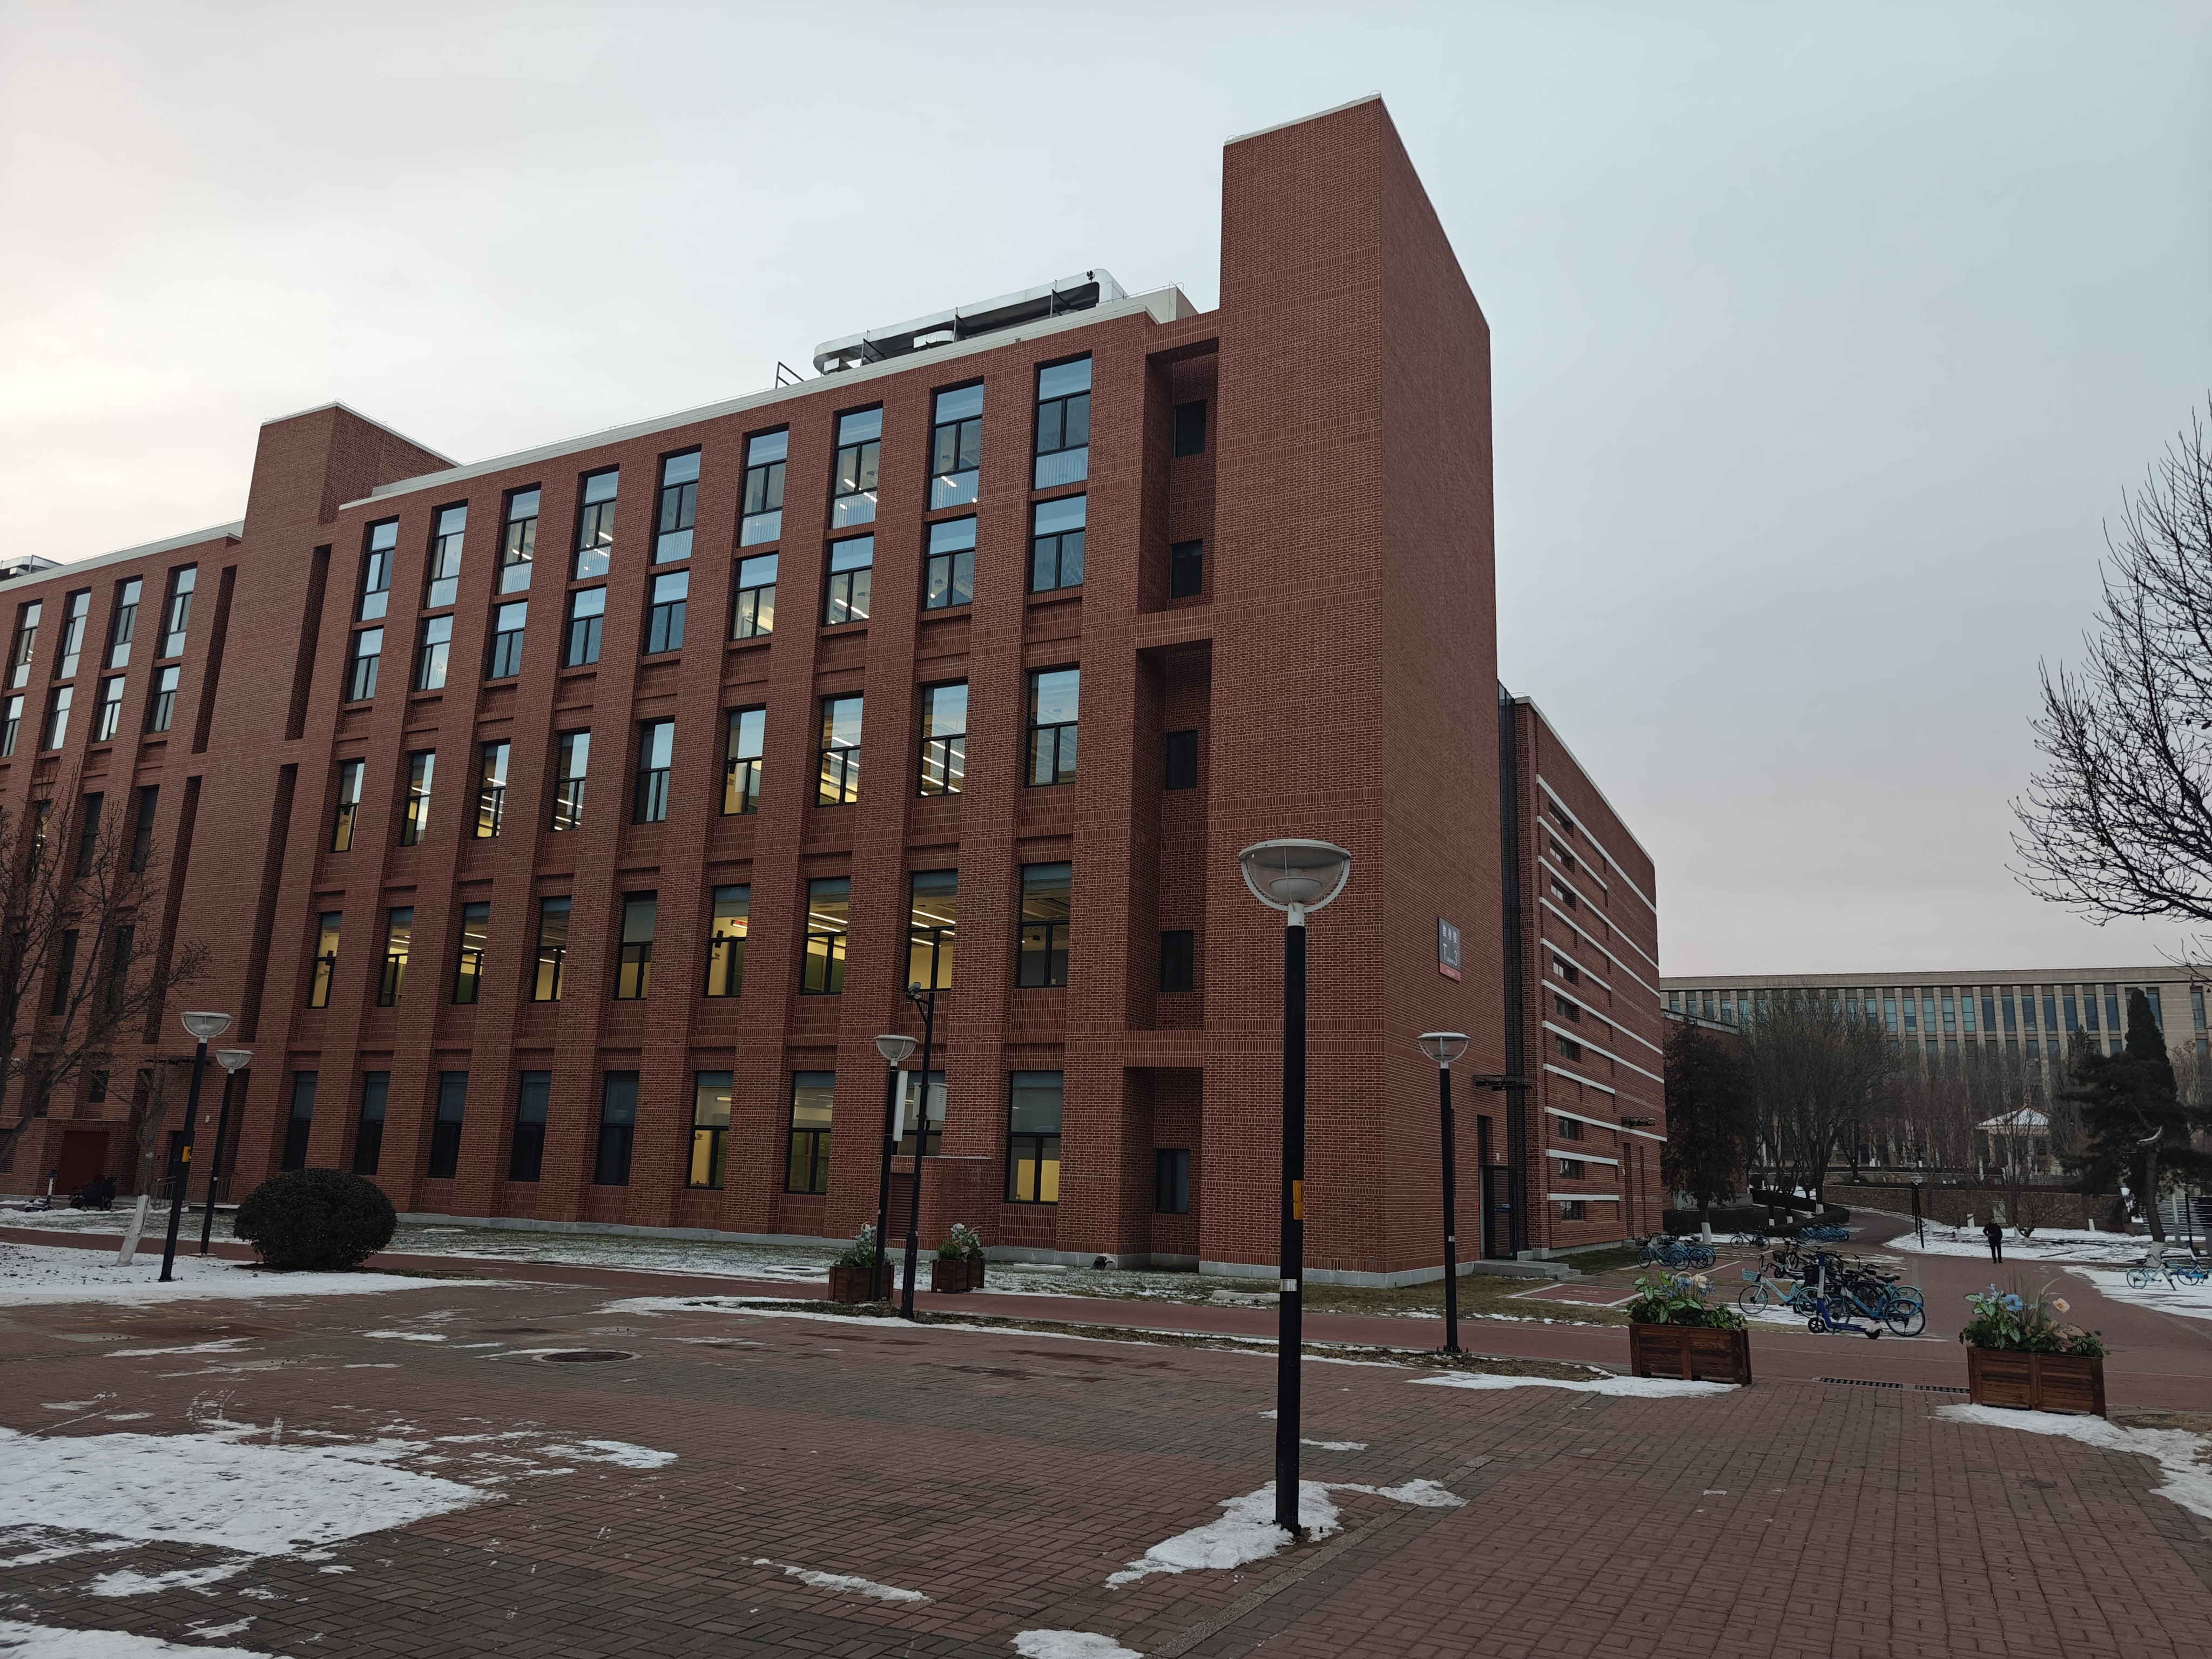
\includegraphics[width=\textwidth]{./data/retri2/mapping/1.jpg}
        \caption{室内场景1 旋转}
    \end{minipage}
    \hfill
    \begin{minipage}[t]{0.48\textwidth}
        \centering
        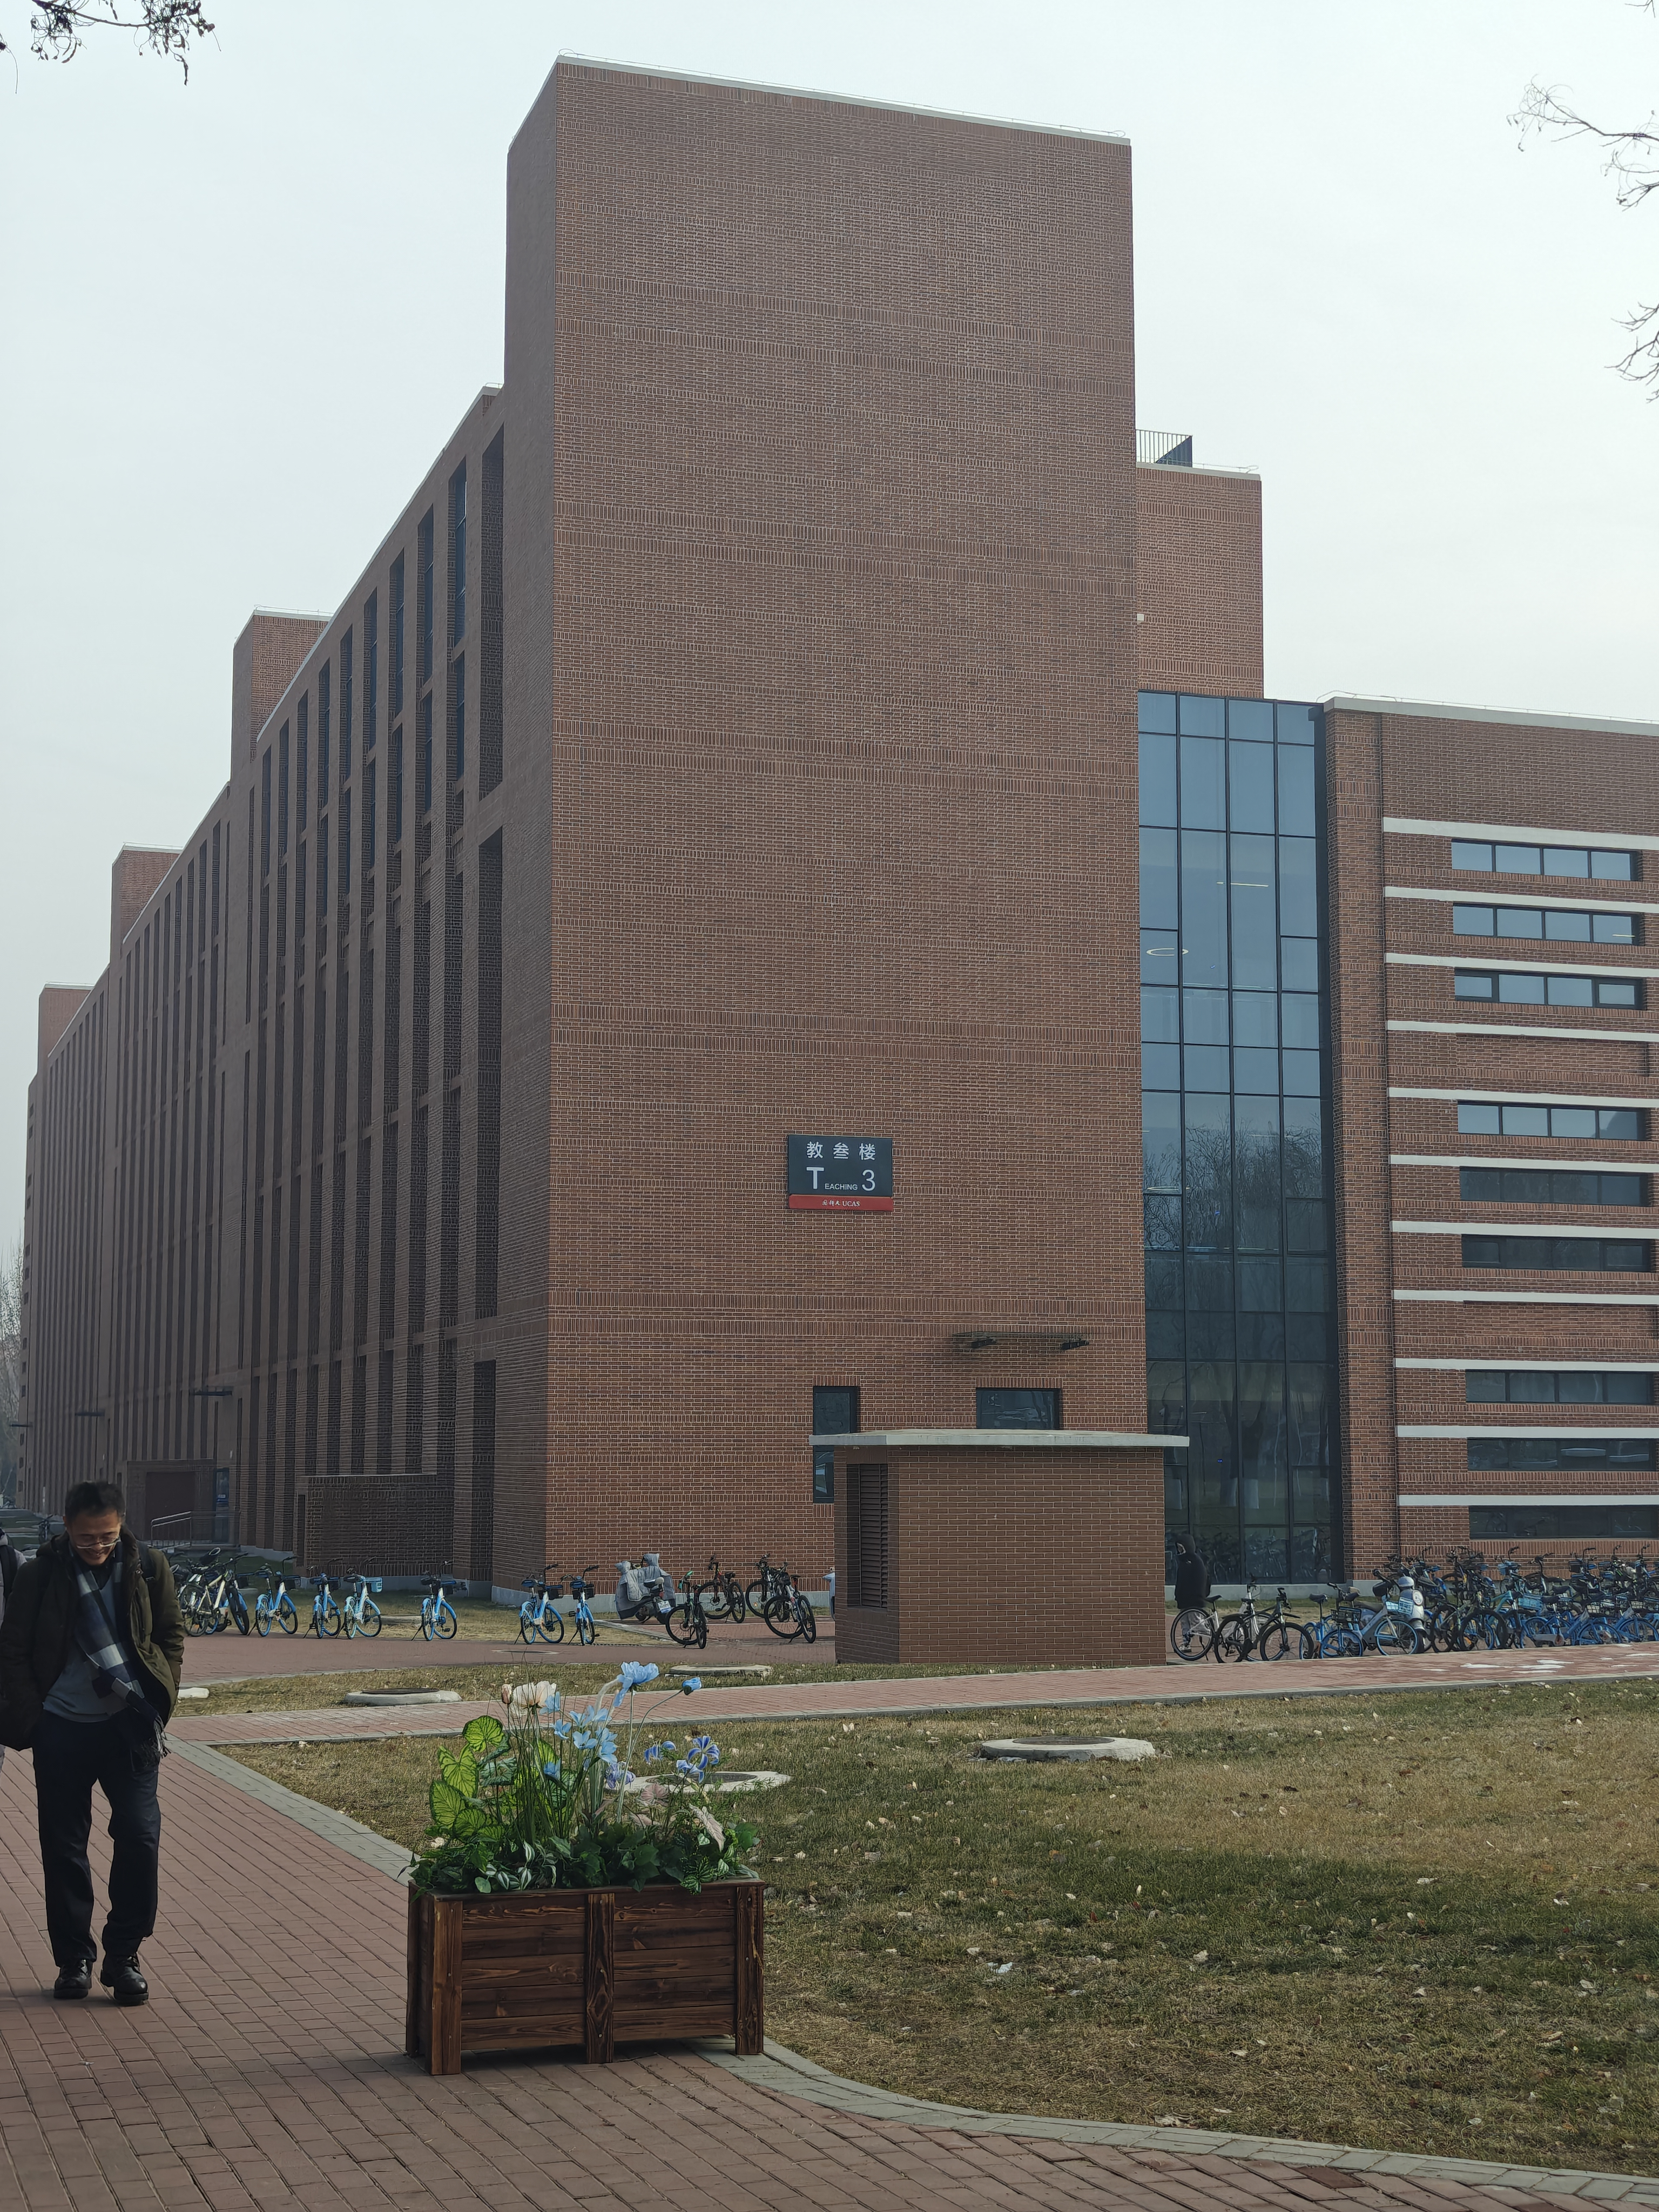
\includegraphics[width=\textwidth]{./data/retri2/mapping/19.jpg}
        \caption{室内场景2 光照变化}
    \end{minipage}
\end{figure}
\begin{figure}[H]
    \centering
    \begin{minipage}[t]{0.48\textwidth}
        \centering
        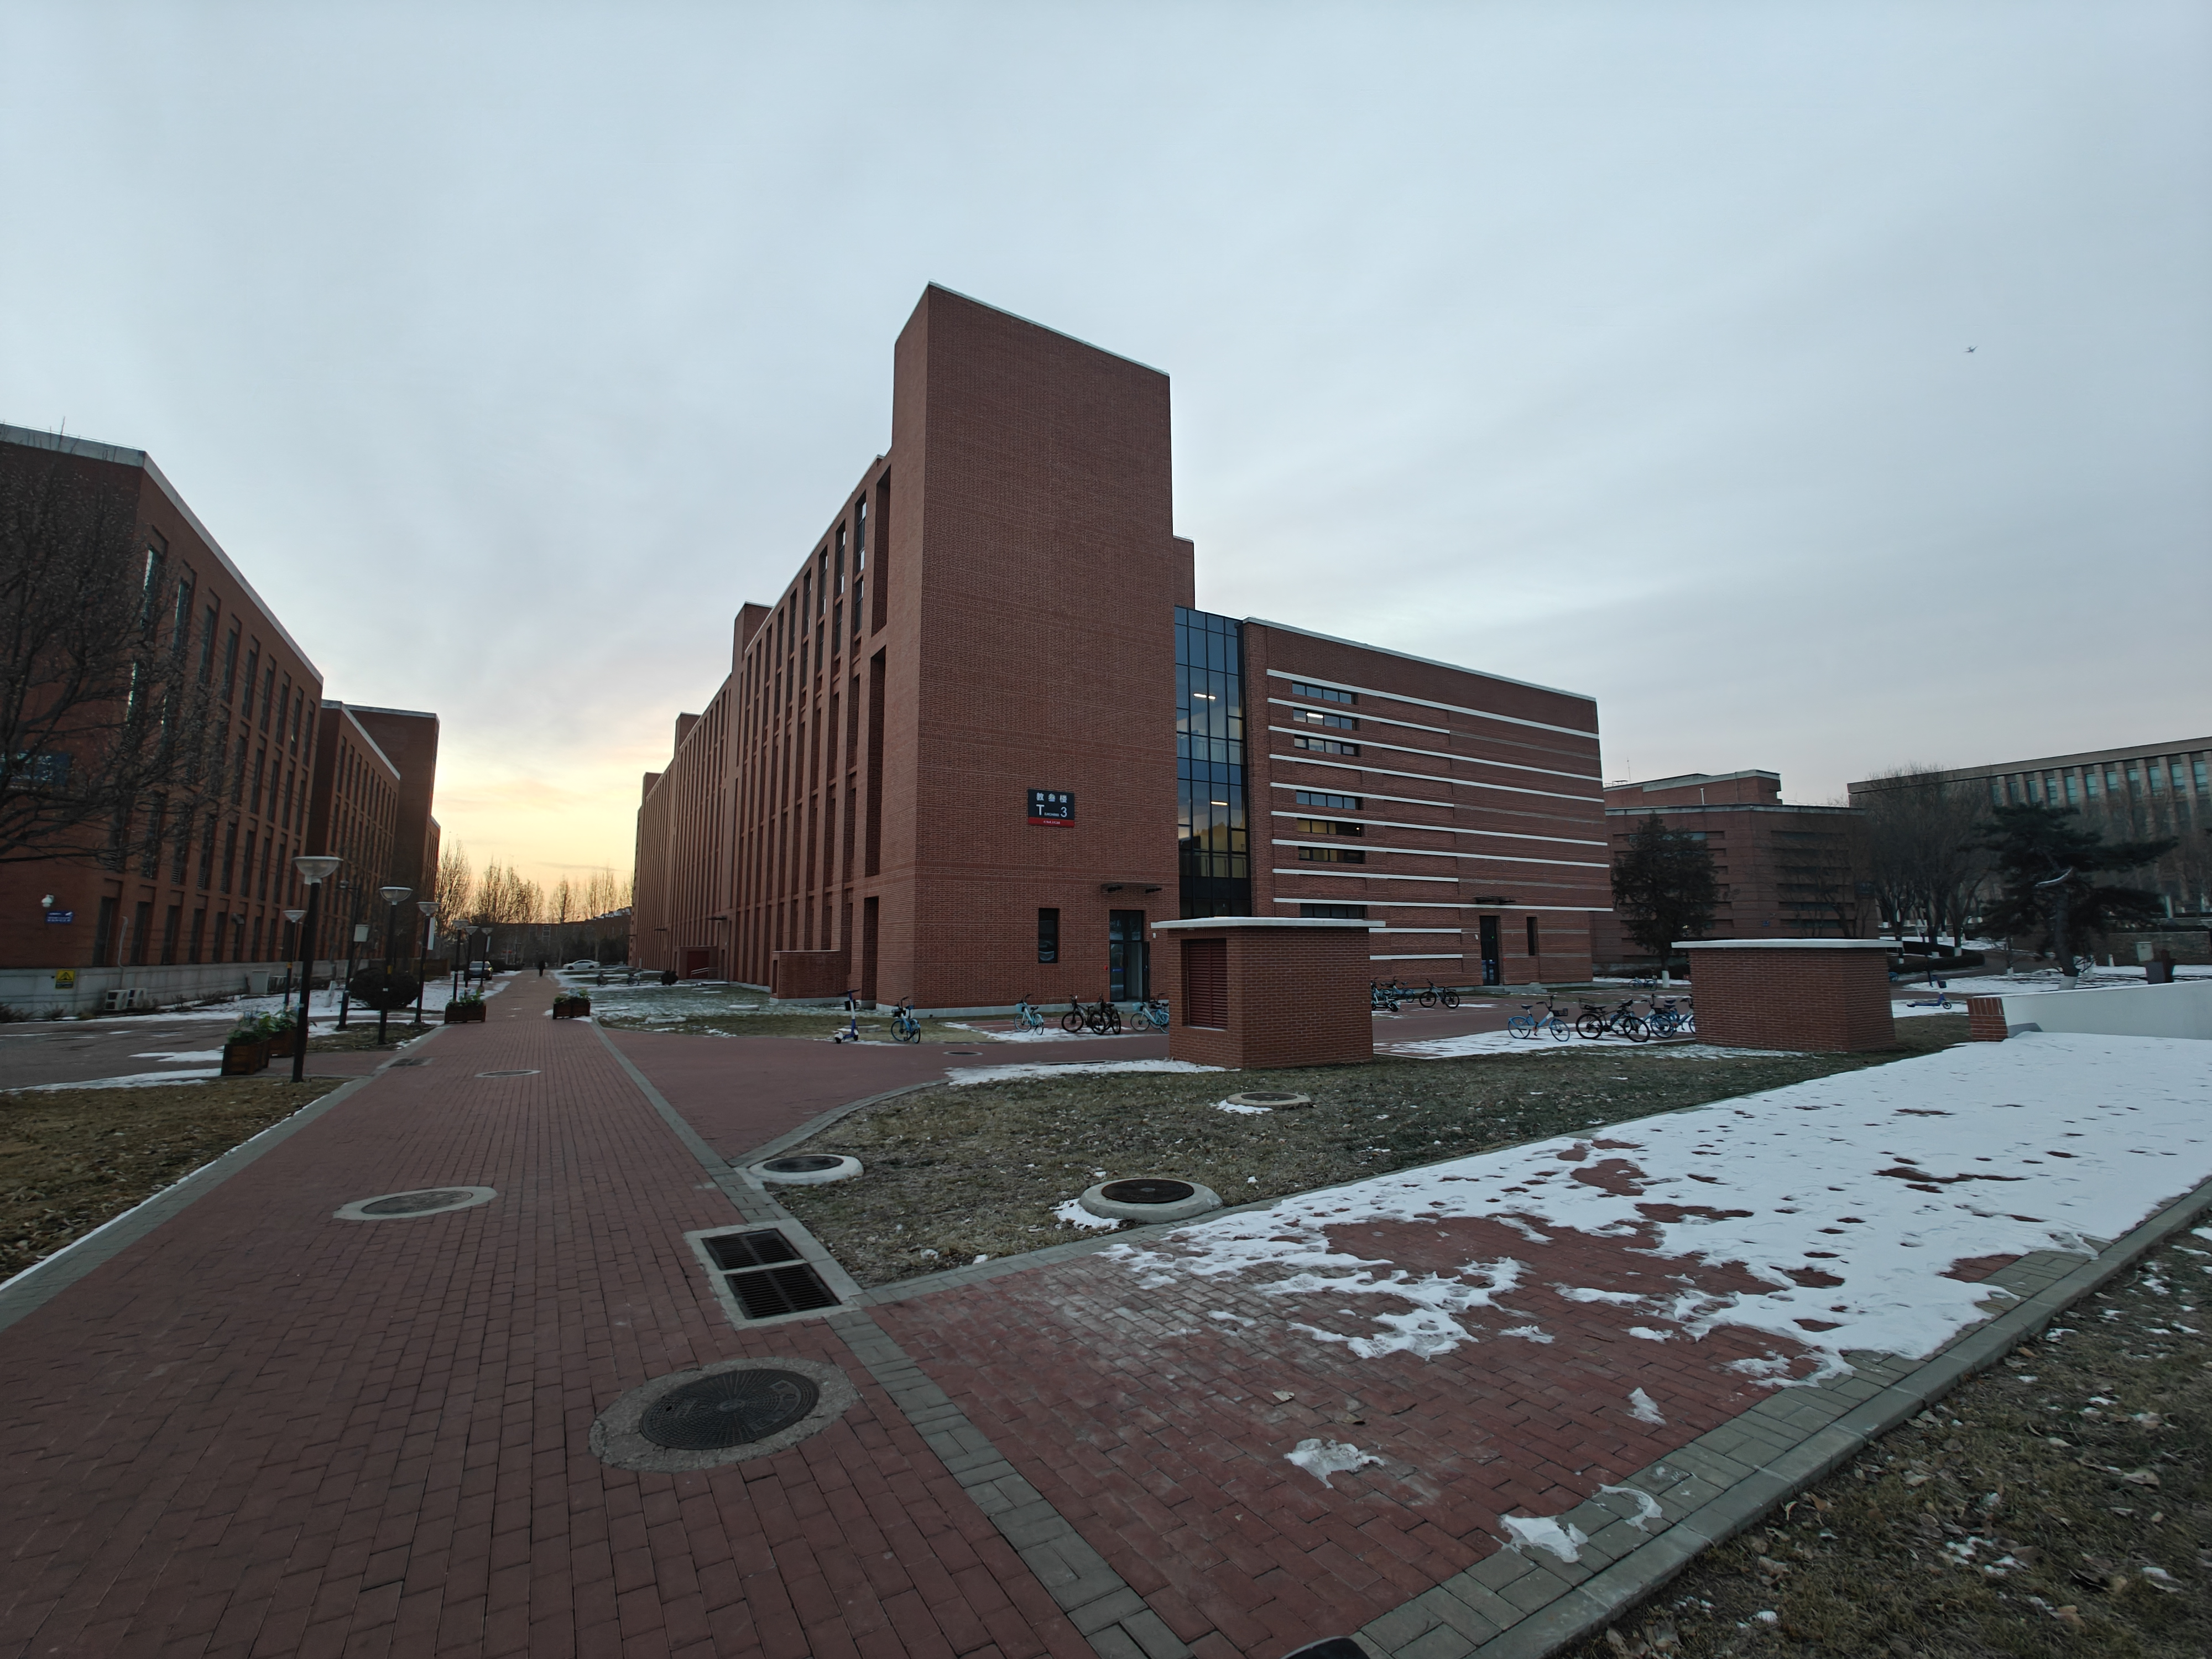
\includegraphics[width=\textwidth]{./data/retri1/mapping/11.jpg}
        \caption{室外场景1}
    \end{minipage}
    \hfill
    \begin{minipage}[t]{0.48\textwidth}
        \centering
        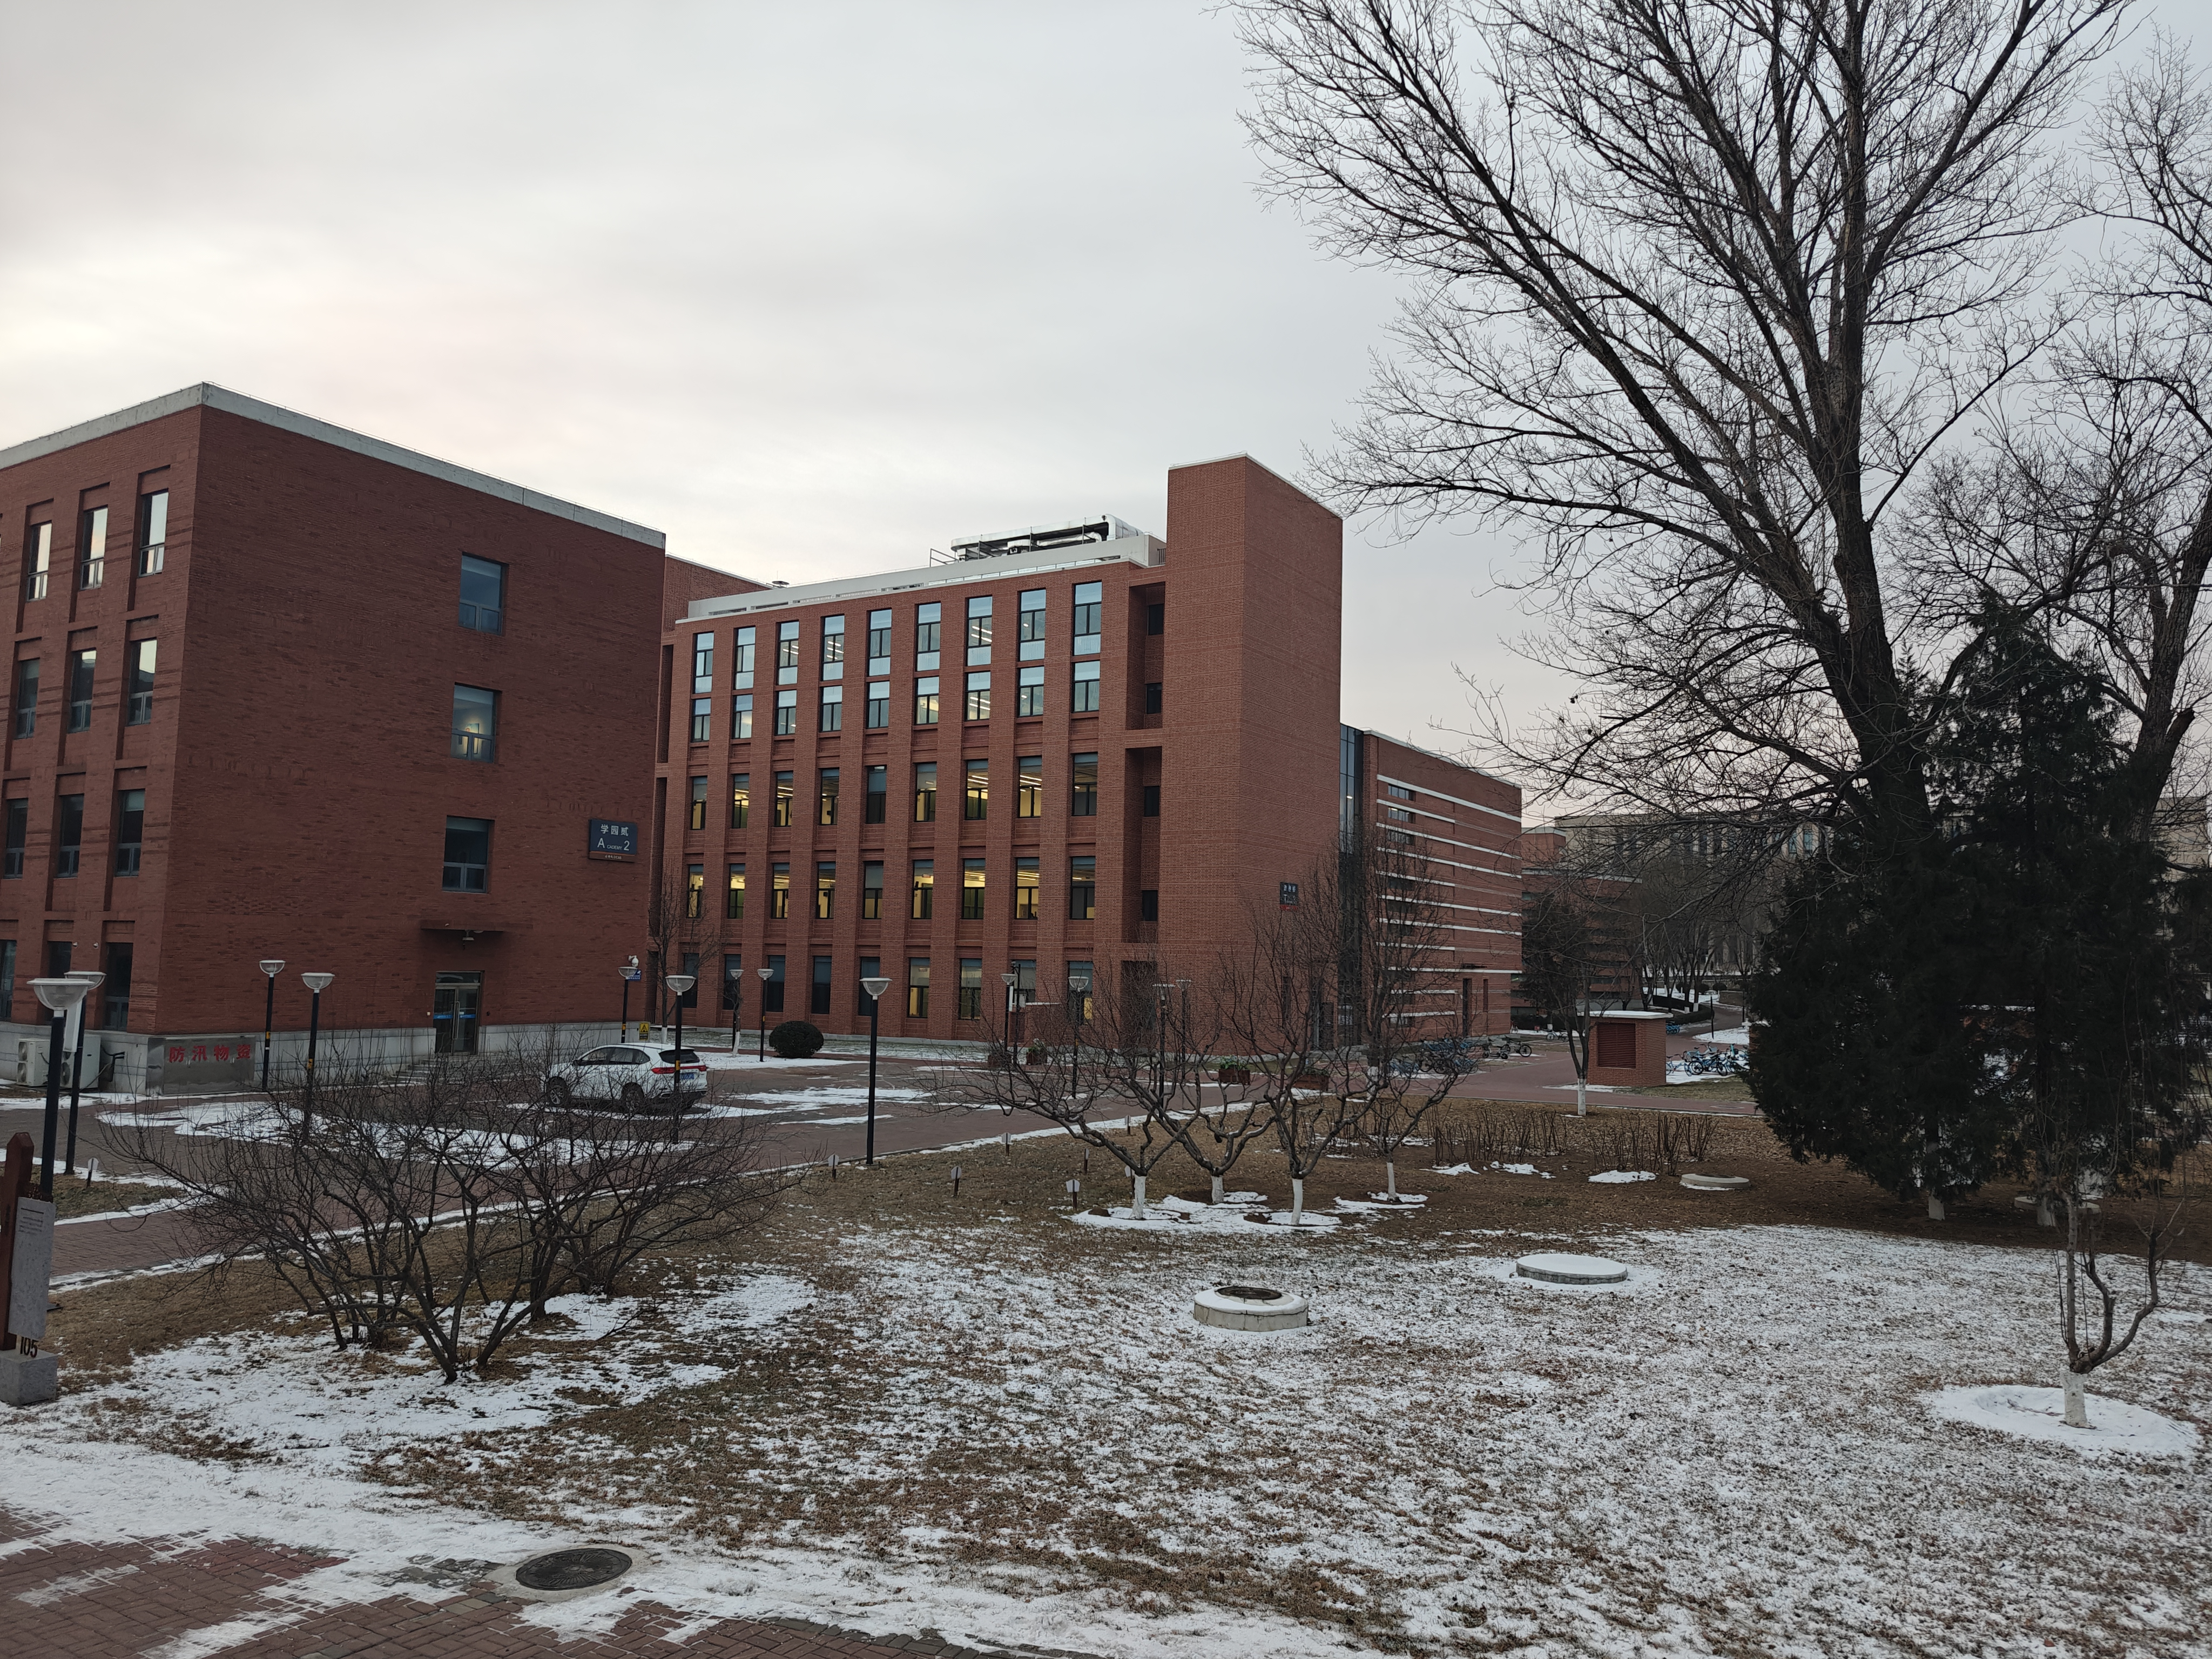
\includegraphics[width=\textwidth]{./data/retri1/mapping/12.jpg}
        \caption{室外场景2}
    \end{minipage}
\end{figure}
\subsection{NetVLAD 检索表现}
列出查询图像及其检索到的 Top-3 结果相似度。
\begin{figure}[H]
    \centering
    \includegraphics[width=0.95\textwidth]{Figure_3.png}
    \caption{室外场景1}
\end{figure}

\begin{figure}[H]
    \centering
    \includegraphics[width=0.95\textwidth]{Figure_4.png}
    \caption{室外场景2}
\end{figure}

\begin{figure}[H]
    \centering
    \includegraphics[width=0.95\textwidth]{Figure_5.png}
    \caption{室内场景1}
\end{figure}

\begin{figure}[H]
    \centering
    \includegraphics[width=0.95\textwidth]{Figure_2.png}
    \caption{室内场景2}
\end{figure}

\subsection{结果具体分析}
\subsubsection{室内场景}
\begin{figure}[H]
    \centering
    \includegraphics[width=0.95\textwidth]{Figure_5.png}
    \caption{室内场景1}
\end{figure}
观察检索结果可知,尽管查询图像存在约45度的倾斜视角及局部遮挡,NetVLAD依然表现出了卓越的视点不变性,Top-3返回结果均为正确场景,且相似度置信度均在0.9999以上。在特征匹配环节,尽管由于视角和尺度的剧烈变化导致视场重叠度降低,使得匹配点数量有所浮动,但整体匹配精度极高。SuperPoint有效地在书脊纹理与架构边缘等高频信息区域建立了正确的对应关系,未出现明显的误匹配现象。这表明SuperPoint学习到的特征描述子具有较强的旋转不变性与抗干扰能力,即便在特征稀疏的极端几何变换下,仍能保证极高的内点率,验证了系统在室内复杂视角场景下的有效性。

\begin{figure}[H]
    \centering
    \includegraphics[width=0.95\textwidth]{Figure_2.png}
    \caption{室内场景2}
\end{figure}
如图所示,本节重点展示了系统在低光照条件下的检索与匹配性能。查询图像采集于室内弱光环境,存在明显的亮度不足与噪声干扰,对特征提取带来了显著挑战。尽管如此,NetVLAD 的检索结果仍表现出很强的语义一致性:Top-1 与 Top-2 均准确召回了同为暗光条件下的图像,相似度达到 1.0000,说明其生成的全局描述子对整体光照强度变化具有较好的鲁棒性。更重要的是,Top-3 成功召回了同一场景在正常光照(开灯/白昼)下的图像,验证了检索算法具备一定的跨域识别能力。

在特征匹配方面,SuperPoint 在低光照同域匹配中表现尤为突出,Top-2 的匹配点数量高达 283 个,表明即便在人眼难以分辨细节的暗区,网络仍能够提取到较为丰富且稳定的纹理特征。在跨光照匹配任务中,尽管局部像素强度发生了明显的非线性变化,算法依然成功获得 28 个高质量关键点匹配,并且匹配连线准确、误匹配较少。这充分展示了 SuperPoint 描述子在应对光照变化时的优越性能,验证了其在实际应用中处理复杂光照条件的潜力。

\subsubsection{室外场景}
\begin{figure}[H]
    \centering
    \includegraphics[width=0.95\textwidth]{Figure_3.png}
    \caption{室外场景1}
\end{figure}
该图展示了室外红砖建筑在不同视角下的检索与匹配效果。Top-1 与 Top-2 结果表明系统对同一场景具有较强鲁棒性:Top-1 在近似视角下获得 348 个高质量匹配点;Top-2 视角更远且存在平移,匹配点降至 27 个,但仍能建立正确的空间对应关系。

需要重点说明的是 Top-3 的误检。尽管 Top-3 并非同一栋建筑,NetVLAD 仍给出很高相似度(0.9999),主要原因在于两者全局外观高度相似:红砖外墙、规则窗户排列以及蓝天背景导致全局描述子发生混淆。同时,SuperPoint 仍产生 11 个匹配点,说明在窗角、砖缝等局部结构相近时,局部描述子也可能出现误匹配。因此,在外观极其相似的场景中,仅依赖匹配点数量作为几何验证依据可能存在误判风险。
\begin{figure}[H]
    \centering
    \includegraphics[width=0.95\textwidth]{Figure_4.png}
    \caption{室外场景2}
\end{figure}
如图所示,该组实验展示了室外红砖建筑场景下的检索与匹配效果。在检索阶段,NetVLAD 取得了较高精度:Top-3 均返回同一建筑目标,相似度得分接近或等于 1.0000,说明其在复杂背景中仍能稳定捕捉场景的整体语义特征。

在特征匹配阶段,SuperPoint 体现出两方面优势。其一是对重复纹理的区分能力:尽管建筑立面存在大量外观相近的窗户阵列,仍能产生几何一致的正确匹配(Top-1 为 146 点,Top-2 为 161 点),未出现明显错配,表明描述子能够融合一定的局部上下文信息以降低重复结构带来的歧义。其二是对非结构化区域的鲁棒性:除建筑刚性边缘外,算法在树枝等形态复杂、不规则区域也能建立稳定对应关系。进一步对比 Top-2(161 点)与 Top-3(69 点)可见,在存在较明显尺度变化(Scale Change)时,匹配点数量虽下降,但关键结构仍被保留,验证了该检索与匹配框架在室外非受控环境下的综合鲁棒性。
\end{document}